La scelta è caduta sui dispositivi mobili. Questa decisione è stata vincolante perchè disponevamo di solo queste risorse \textit{hardware}.

\section{Sviluppo applicazione iOS}
\subsection{Conversione del modello da Keras a CoreML}
\textbf{tempo di lavoro:} 12 giorni\\
\newline
Per poter usare il modello pre-addestrato sul cellulare abbiamo dovuto convertirlo nel formato \textit{.mlmodel} in modo da poter usare il \textit{framework Core ML}.\\
\newline
\textbf{Problemi riscontrati:} durante la conversione del modello sono apparsi diversi errori che impedivano la conversione. Gli errori sono simili a quello riportato di seguito:
\begin{figure}[H]
	\centering
	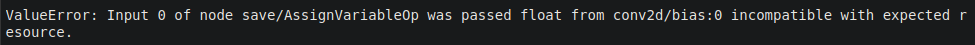
\includegraphics[scale=0.60]{./images/img1.png}
\end{figure}
\textbf{Soluzioni provate:}
\begin{itemize}
	\item Abbiamo preso spunto dal codice che si trova sul blocco di lucidi visti a lezione. Esso usa il package \textit{tfcoreml}. Il focus dello \textit{script} è il seguente:
	
	\pythonexternal{./codes/coreml1.py}
	
	A questo punto serviva ottenere il file in formato \textit{.pb} da usare come \textit{input}. Questo file prende il nome di modello congelato. Prima di ottenerlo serve salvarci il modello che si ottiene con \textit{Tensorflow}. Esso è formato da quattro file:
	\begin{itemize}
		\item \textbf{model-ckpt.meta}: contiene il grafico completo (flusso di dati, le annotazioni per le variabili, le \textit{pipeline} di \textit{input} e altre informazioni);
     	\item \textbf{model-ckpt.data-0000-of-00001}: contiene tutti i valori delle variabili (pesi, segnaposto, gradienti, iperparametri, ecc.);
     	\item \textbf{model-ckpt.index}: ci sono tutti i metadati. È una tabella immutabile in cui ogni chiave è un nome di un tensore e il suo valore descrive i metadati di un tensore;
     	\item \textbf{checkpoint}: tutte le informazioni sul \textit{checkpoint}.
	\end{itemize}
      
	\pythonexternal{./codes/coreml2.py}
	
	\textit{estimator\_model.train} serve a verificare che il modello esportato in precedenza sia effettivamente funzionante.\\
	\newline
	Il modello congelato ci consente di eliminare tutte le informazioni in più che vengono salvate perchè si potrebbe ricaricare quello appena salvato e l'addestramento continua da dove era stato interrotto.
	
	\pythonexternal{./codes/freezer.py}
	
	\item Uno dei nuovi tentativi si è basato sul cambio di codice per salvare il modello: abbiamo usato il seguente codice:
	
	\pythonexternal{./codes/coreml3.py}
	
	Tuttavia, i risultati non sono stati quelli sperati.
	
	\item Cercando nella documentazione di \textit{coreml}, abbiamo scoperto che non sono previsti più aggiornamenti e consigliavano di usare un nuovo \textit{package}. Anche se fossimo stati in grado di convertirlo non avremmo potuto utilizzato su sistemi operativi \textit{iOS} maggiori di 12. La nuova libreria che abbiamo usato si chiama \textit{coremltools}.
	
	\pythonexternal{./codes/coremltools.py}
	
	\item Per non avere altri errori che ci apparivano, abbiamo usato i livelli di convoluzione presi direttamente da \textit{keras} e non da \textit{tensorflow}. E' stato molto difficile superare tutti questi ostacoli perché i messaggi di errore non aiutavano a capire bene che cosa bisognasse modificare.
	
	\item Successivamente, per aumentare l'accuratezza, è stata inserita una funziona di attivazione personalizzata. Purtroppo, anche con \textit{coremltools} non siamo stati in grado di convertirlo perchè ci appariva un errore in corrispondenza del livello della nuova funzione:
	
	\begin{figure}[H]
		\centering
		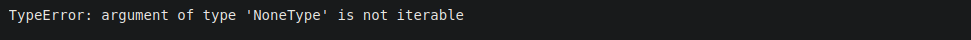
\includegraphics[scale=0.60]{./images/img11.png}
	\end{figure}
	
\end{itemize}
\textbf{Soluzione finale:} abbiamo deciso di usare \textit{Tensorflow Lite} perchè siamo riusciti a convertire il modello subito senza nessun problema.

\subsection{Conversione del modello da Keras a Tensorflow Lite}
\textbf{tempo di lavoro:} 1h\\
\newline
Come accennato nel paragrafo precedente, abbiamo convertito il modello usando \textit{Tensorflow Lite}.
\pythonexternal{./codes/tensorflowLite.py}
Il seguente codice consente di caricare il modello addestrato tramite \textit{Tensorflow} e di convertirlo nel formato .\textit{tflite} pronto per essere usato su un dispositivo mobile nel nostro caso.

\subsection{Sviluppo applicazione con Swift 5 e Xcode 12}
\textbf{tempo di lavoro:} 20 giorni\\
\newline
\textit{Swift} è un linguaggio di programmazione \textit{object-oriented} concepito per programmare sui sistemi operativi \textit{Apple}.\\
\newline
\textit{Xcode} è un ambiente di sviluppo integrato completamente sviluppato e mantenuto da \textit{Apple}, che consente di sviluppare \textit{software} per i sistemi \textit{macOS}, \textit{iOS}, \textit{watchOS} e \textit{tvOS}.\\
\newline
Abbiamo dovuto prendere un pò di familiarità con il nuovo linguaggio e il nuovo \textit{IDE} dato che non avevamo mai programmato nel mondo \textit{Apple}. La documentazione messa a disposizione agli sviluppatori è molto vasta e le solide basi apprese a ingegneria hanno fatto il resto.
La scelta è ricaduta direttamente sia all'ultima versione del linguaggio che dell'ambiente di sviluppo perché non avevamo vincoli sulla realizzazione dell'applicazione.\\
\newline
Le interfacce si realizzano in modo molto semplice perchè \textit{Xcode} consente di spostare gli elementi grafici con il \textit{mouse} e di posizionarli come si vuole. Tuttavia, è stata la parte che ha richiesto più tempo perchè li abbiamo dovuti configurare nel modo più adatto alle nostre esigenze. 
\begin{figure}[H]
	\centering
	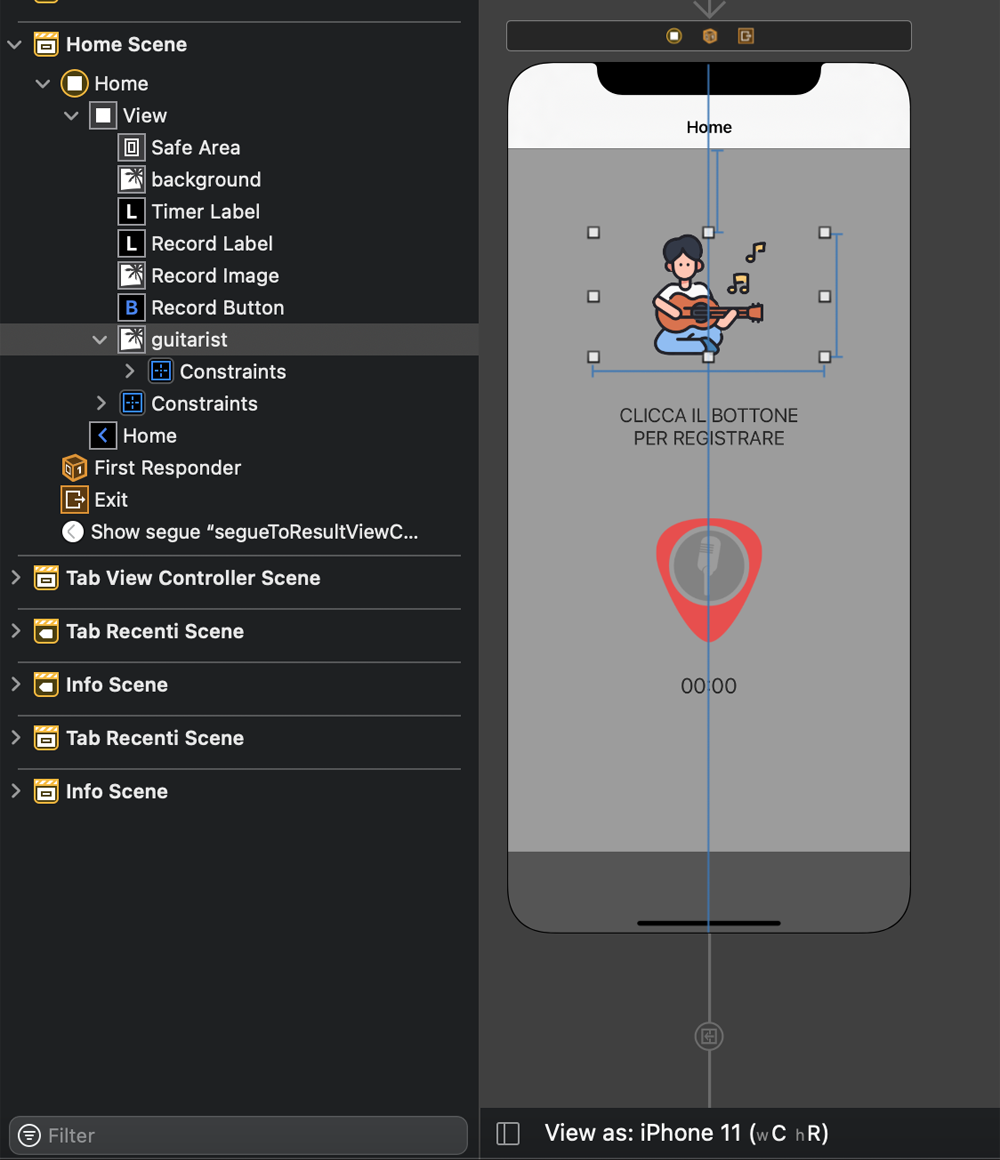
\includegraphics[scale=0.20]{./images/img2.png}
\end{figure}
E' stata prestata anche molta attenzione a rendere compatibile l'applicazione su modelli diversi. La dimensione dello schermo influisce molto sul \textit{layout} dell'applicazione. Senza le giuste modifiche è possibile che un elemento venga nascosto o spostato.
\begin{figure}[H]
	\centering
	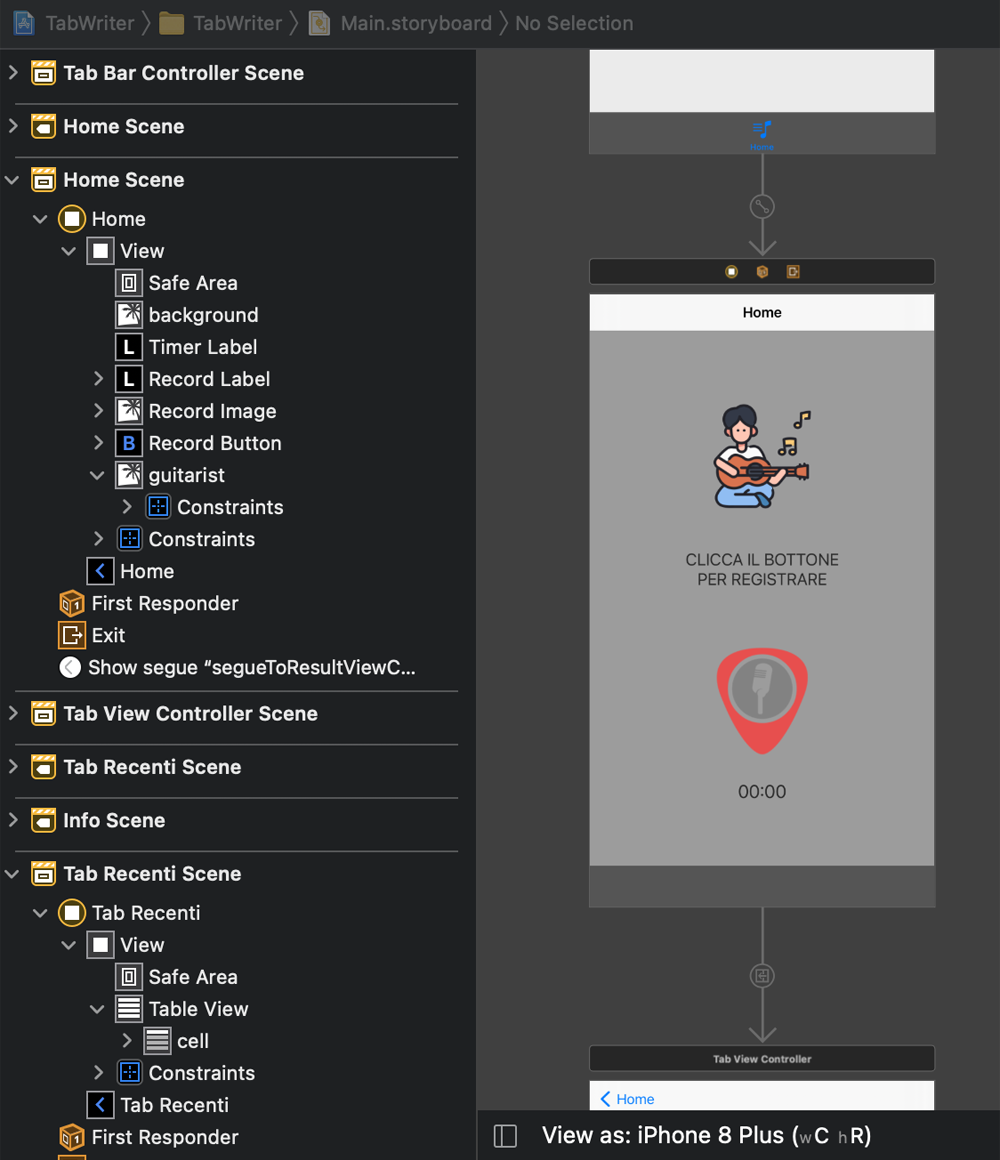
\includegraphics[scale=0.20]{./images/img3.png}
\end{figure}
Le due immagini precedenti mostrano chiaramente quello appena descritto: i due dispositivi sono diversi e le proporzioni vengono rispettate in entrambi.\\
\newline
Inoltre, una particolare attenzione è stata dedicata anche sulla nuova modalità che sta riscontrando un grandissimo successo: la \textit{dark mode}. Dunque, sono stati presi tutti gli accorgimenti necessari per avere sia l'app compatibile con la versione chiara che con quella scura. L'immagine successiva mostra l'app in versione \textit{dark}:
\begin{figure}[H]
	\centering
	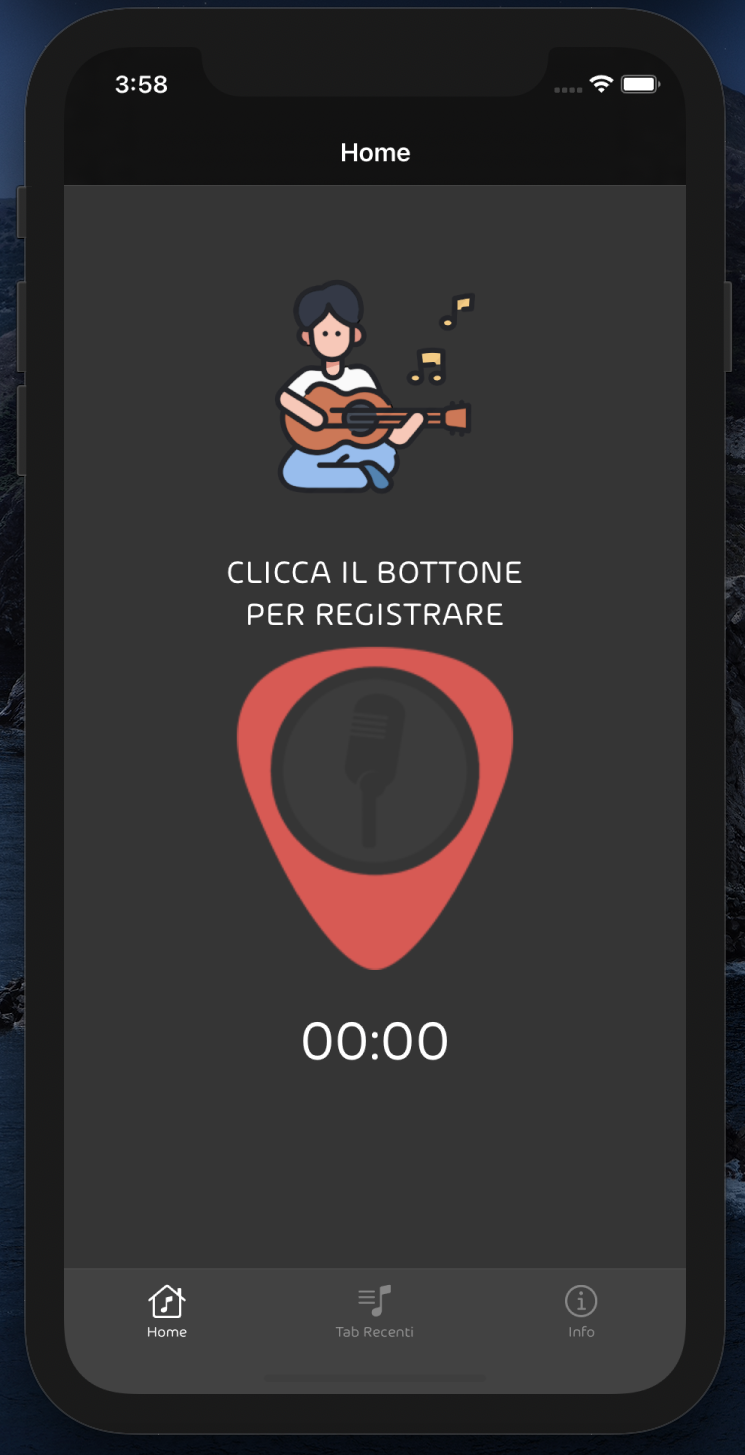
\includegraphics[scale=0.20]{./images/img10.png}
\end{figure}

\subsection{Uso di TensorFlow Lite su iOS}
Abbiamo eseguito i seguenti passaggi:
\begin{itemize}
	\item Registrato l'\textit{app} sul sito \textit{Firebase} perchè bisogna monitorarla (passaggio obbligatorio come scritto nella guida);
	\item Scaricato e aggiunto il file di configurazione che si ottiene dopo la registrazione su \textit{Firebase};
	\item Aggiunto \textit{Firebase} all'\textit{app};
	\item Inizializzato \textit{Firebase} nel progetto \textit{iOS} e usate le sue \textit{API} per usare il modello sullo \textit{smartphone}.
\end{itemize}

\subsection{Uso di un server per l'uso della libreria Librosa}
\textbf{tempo di lavoro:} 5 giorni\\
\newline
\textbf{Problemi riscontrati:} putroppo non sono state trovate librerie in grado di convertire il file audio nella trasformata a Q costante.\\
\newline
%
\textbf{Soluzioni provate:}
\begin{itemize}
	\item Abbiamo provato ad usare la libreria \textit{PythonKit} senza successo perchè sui dispositivi \textit{iOS} manca l'interprete \textit{Python}.\\
\end{itemize}
%
\textbf{Soluzione finale:} per questo motivo ci siamo serviti di un \textit{server} che prende in ingresso la registrazione che è stata effettuata dallo \textit{smartphone} e restituisce in uscita le immagini del file audio. Ovviamente la soluzione non è efficiente ma ai fini del progetto può andare più che bene. La predizione viene eseguita sul dispositivo e \textbf{non} sul \textit{server}.\\
\newline
Il \textit{server} è stato scritto grazie al \textit{framework} di \textit{Python} che si chiama \textit{flask}

\pythonexternal{./codes/flask.py}

\section{Sviluppo applicazione Android}
\subsection{Conversione del modello da Keras a Tensorflow Lite}
\textbf{tempo di lavoro:} 1h\\
\newline
Tutto ha funzionato al primo colpo senza nessun problema.\\
\pythonexternal{./codes/tensorflowLite.py}
Il seguente codice consente di caricare il modello addestrato tramite \textit{Tensorflow} e di convertirlo nel formato .\textit{tflite} pronto per essere usato su un dispositivo mobile nel nostro caso.

\subsection{Sviluppo applicazione con Java 1.8 e Android Studio 4.1.2}
\textbf{tempo di lavoro:} 12 giorni \\
\newline
\textit{Java} è una piattaforma che consente di eseguire i programmi scritti in questo linguaggio.\\
\newline
\textit{Android Studio} è un ambiente di sviluppo integrato per lo sviluppo per la piattaforma \textit{Android}.\\
\newline
L'applicazione che è stata realizzata da un punto di vista estetico è uguale a quella su \textit{iOS}. Cambiano solo leggeri particolari che differenziano i due mondi.\\
\newline
\textbf{Problemi riscontrati:} putroppo non sono state trovate librerie in grado di convertire il file audio nella trasformata a Q costante.\\
\newline
%
\textbf{Soluzioni provate:}
\begin{itemize}
	\item Abbiamo usato la soluzione del \textit{server} come in \textit{iOS}.\\
\end{itemize}
%
\textbf{Soluzione finale:} grazie ai ricevimenti fatti con il professore, ci è stato consigliato di usare \textit{chaquopy}.